\chapter{机器学习基础}
\label{chap:5}
%%%%%%%%%%%%%%%%%%%%%%%%%%%%%%%%%%%%%%%%%%%%%%%%%%%%%%%%%
%%%%%%%%%%%%%%%%% author:dormir_yin %%%%%%%%%%%%%%%%%%%%%
%%%%%%%%%%%%%%%%% part:5.1          %%%%%%%%%%%%%%%%%%%%%
%%%%%%%%%%%%%%%%%%%%%%%%%%%%%%%%%%%%%%%%%%%%%%%%%%%%%%%%%

深度学习其实也是机器学习的一个分支。为了更好的理解深度学习,我们必须也要了解一下机器学习的基础知识。这章给大家简要介绍了机器学习中一些重要的概念,这些内容在本书的后续章节会涉及到。如果你是初学者或者想对机器学习有更深入的了解,推荐你找一本机器学习的教科书。比如说Murphy(2012)或者Bishop(2006)。如果你已经对机器学习的基础知识比较熟悉了,你可以直接开始看5.11。那部分内容介绍的我们为何从传统机器学习转向深度学习算法,或者说传统的机器学习如何影响深度学习的。

这章开始,我们首先会先定义一下什么是机器学习算法。随后我们会给一个机器学习算法的例子 线性回归算法。接着我们介绍拟合训练数据和为某个训练好的模型泛化(generalize)到新的数据集的不同之处。大部分机器学习算法会让我们设置超参数(hyperparameters)。这些超参数是需要我们自己额外定义的,而不能通过机器学习算法在训练过程自动优化。我们会讨论如何利用额外的数据设置超参数。机器学习本质上就是应用统计学。和应用统计学不同的是它强调了了利用计算机来对一些复杂的函数进行统计估计。但是弱化了对估计出来的函数计算置信区间的要求。就是说它利用统计学方法的得出一个模型,但它不强调用传统的假设检验的方式来对该模型进行评估。接着我们会介绍两个核心的统计算法:频率估计(frequentist estimator)和贝叶斯推断(Bayesian inference)\footnote{频率学派和贝叶斯学派也是统计学的两大流派。}。大部分机器学习任务可以分为监督学习和无监督学习两类。我们会对这两类做一个介绍,同时会介绍一些常见属于这些类别的机器学习算法。大部分深度学习算法是基于一种叫随机梯度下降法(stochastic gradient descent)的优化算法。我们会介绍如何构建一个完整的机器学习算法,机器学习算法包含多个部分:优化算法,损失函数,模型和数据集。最后,在\ref{sec:5.11}我们介绍了传统机器学习算法遇到的一些困难,一些因素限制了传统机器学习算法的发展。这些困难促使我们发展深度学习来解决传统机器学习算法所不能解决或者很难解决的问题。

\section{机器学习算法}
\label{sec:5.1}

所谓机器学习算法,就是能够从数据中自我学习的算法。但是学习到底是什么含义?Mitchell(1997) 提供了一个定义。在讲这个定义之前我们先介绍机器学习所涉及的几个名词:学习的任务(Task)$T$, 经验(Experience)$E$, 对模型的评估准则(Performance measure)$P$。现在我们可以给出这个定义了:如果一个计算机程序针对任务$T$, 它的表现可以通过$P$ 来评估,并且模型本身可以根据$E$来改进,那么我们就说这个程序可以从经验$E$中来“学习”。

我们可以想象,经验(E) 任务(T) 还有评估策略(P)可以有很多不同的形式,在这本书中不会给这些名词一个正式的定义。但是我们在接下来的部分中会对它们进行大致的描述,并给一些例子来帮助大家理解这些名词,已经如何用它们来构建一个机器学习算法。

\subsection{任务(Task) $T$}
\label{sec:5.1.1}
机器学习可以解决一些传统的算法很难解决的问题,因为之前我们总会用人为设计的固定的算法来解决问题。从一个科学或者哲学的观点来看,机器学习之所以有趣,是因为在发展理解机器学习算法的同时,我们也会思考发现人类智能的本质。去了解人是如何思考的。

在这一段,我们会给任务 $T$ 一个相对正式的定义。学习本身的过程不能称之为任务,学习的目的是为了获得完成任务的能力。举个例子: 如果我们制作出了一个机器人,想让它具有走路能力,那么走路就是任务$T$。我们可以写一个程序让机器人自己学习如何走路(机器学习),也可以直接写一个程序直接控制机器人走路(传统算法)。

机器学习任务通常描述了机器学习系统如何处理一个个\textbf{数据实例( Example)}\footnote{译者注:有时也会翻译成数据点}。实例是特征的集合。这些特征来自于我们设计的机器学习系统需要处理的事件或者物体,而且都已经被量化了。我们通常把实例表示成一个向量$x\in \mathbb{R}^{n}$,向量的每个元素$x_i$表示不同的特征。比如说图像的特征通常就是图像的像素值。

机器学习可以解决很多不同的任务。下面我列举了最常见的机器学习任务:
\begin{itemize}
\item \textbf{分类(Classification):} 在这个任务中,计算机算法需要对输入进行分。假设总共有$k$类,判断每个输入属于哪个类别。为了完成这个任务,学习算法通常需要构建一个函数,或者叫对应关系:$f:\mathbb{R}^{n}\rightarrow \{1,...,k\}$。模型会将每个输入$x$对应到某个类别$y$。当然也有很多其它的分类任务,比如说$f$不输出类别而是输出一个概率分布,每个类别对应一个概率。分类任务一个常见例子就是物体识别(object recognition)。在这个例子中,我们的输入是一幅图片(通常是像素值的集合)。输出是图片中物体对应的编码。比如说Willow Garage PR2 机器人 就可以识别不同的饮料,并把他们送给点单的客人(Good-fellow et al., 2010)。目前最好的目标识别算法就是通过深度学习实现的(Krizhevsky et al., 2012; Ioffe and Szegedy, 2015)。同时,目标识别算法也可以用于人脸识别,这样我们就可以对照片里的每个人进行自动标注了,而且也可以帮助计算机更好的和人类进行交互。

\item \textbf{缺失特征情况下的分类:} 如果一些数据实例中某些特征不确定,分类问题会变得比较难。也就是说不能保证输入向量$x$里每个对应的特征都可以提供。不同的数据实例$x$缺失特征也有可能不一样。传统的分类任务中,学习算法需要定义一个函数,将输入向量映射到一个输出类别。但如果一些输入特征缺失了,学习算法就需要定义一系列函数,每个函数的输入特征是原输入向量的一个子集(去掉了缺失的向量)。这类任务在医疗诊断中出现的越来越多。因为很多医疗测试很昂贵,有的还对身体有害。为了高效地来定义这一系列函数,我们可以对所有的相关变量来学习一个概率分布,在分类的时候我们就可以求解边缘概率的方法来把缺失值给去掉\footnote{编者注:在这个方法中每个特征都被看作是一个变量。为了更好的理解先看一下边缘概率的定义}。最后我们也只需要定义一个函数来描述联合概率分布。 Goodfellow et al. (2013b) 介绍了一个详细的例子。很多这小结介绍的其它的任务也可以被看成处理缺失的某些特征的数据。缺失特征情况下的分类只是机器学习所0能完成任务的一个例子。

\item \textbf{回归(Regression):}  在这类任务中,计算机程序需要根据输入预测一个数值。为了解决这个问题,学习算法需要构建一个函数$f:\mathbb{R}^{n}\rightarrow \mathbb{R}$ 这类任务和分类任务很像,唯一的不同就是输出的格式不一样,分类任务要求输出的是输入对应的类别,是离散的,而回归任务要求的输出是连续的数值。回归任务的一个例子就是保费的计算,保险公司需要求一下投保人未来索赔的期望来确定他需要交多少保费。当然预测证券未来的价格也是回归任务的一种。回归预测也可以用于程序交易。

\item \textbf{描述(Transcription):}  在这类任务中,机器学习系统需要观察一些非结构化数据,然后用文字或者离散化的符号描述它们。比如说文字识别,计算机程序需要识别出图片中所包含的文字,然后将识别出来的文字返回。比如说谷歌街景(Google Street View)就是利用深度学习来处理街道号码的(Goodfellow et al.,2014d)。另一个例子是语音识别,计算机程序会根据输入的波形来判断我们说的话。然后将它们转成文字或者文字对应的编码。现在深度学习是语音识别系统一个非常重要的组成部分,已经被好多大公司使用,包括微软,IBM,谷歌(Hinton et al.,2012b)。

\item \textbf{机器翻译(Machine translation):}  在机器翻译任务中,我们需要将某种语言的序列翻译成另一种语言的对应的序列。这是自然语言处理的的一部分,比如说将英语翻译成法语。深度学习在这些任务中,表现的越来越出色(Sutskever et al., 2014; Bahdanau et al., 2015)。
\item \textbf{结构化输出(Structured output):} 这类任务一般都要求输出是一个向量(或者其他能够存储多个值的数据结构)和向量中不同元素之间的关系。这样的任务太多了,包括我们上面提到的描述和机器翻译。当然还有一些其他的任务,比如说通过语法分析将一个句子映射成为一个语法树。这棵树需要可以表现句子的语法结构,并且每个树节点都要标注词性:动词,名词,副词等等。Collobert (2011)介绍了一个通过深度学习进行语法分析的例子。另一个例子是图像的像素分割(pixel-wise segmentation),在这个例子中,程序需要给每个像素点一个特定的类别。举个例子,深度学习可以用来标注卫星照片中道路的位置(Mnih and Hinton, 2010)。在这类任务重,输出的格式不需要和输入的格式一样。比如说图像描述(image captioning),计算机程序需要观察一幅图像然后输出一个句子来描述这幅图像(Kiroset al., 2014a,b; Mao et al., 2015; Vinyals et al., 2015b; Donahue et al., 2014;Karpathy and Li, 2015; Fang et al., 2015; Xu et al., 2015)。我们之所以叫结构化输出是因为,程序的输出是有内在联系的。比如说图像描述任务中我们必须要输出一个符合语法规范的句子,而不能仅仅是字母的随机组合。

\item \textbf{异常检测(Anomaly detection):}  在这类任务中,计算机程序会对输入的事件和目标进行筛选,找出那些异常的的事件或者事物。信用卡欺诈检测就是这类任务的一个例子。通过对你的消费习惯进行建模,当你的卡被盗刷的时候,信用卡公司可以检测你的信用卡是否被盗刷了。当小偷盗取了你的行用卡或者信用卡信息,他进行消费的时候,这些消费记录会和你的消费习惯的概率分布不一致。这样信用卡公司在检测到你的信用卡账号有异常购买记录的时候就会直接把你的信用卡给锁了。可以看一下Chandola et al. (2009),里面介绍了一些异常检测的方法。

\item \textbf{模仿合成及采样(Synthesis and sampling):}  在这类任务中,机器学习算法需要生成一些和训练数据相似的数据。这类任务在艺术和多媒体领域很有用,艺术家进行创造的过程是很枯燥的,而且要花费大量的时间精力。比如说,在电脑游戏中,我们可以自动生成一些物品纹理和风景。而不是依靠艺术家一点一点画出来(Luo et al., 2013)。当然我们也可以通过输入产生一些比较特殊类别的输出。比如说语音合成,我们输入一个句子,然后程序就会合成这个句子对应的语音波形。这也是上文提到的结构化输出任务,但是在这个任务中每个输入并没有对应的唯一的正确的输出。我们期望输出会有多一点的变化,这样就会让人感觉更加自然和真实。

\item \textbf{缺失值预测(Imputation of missing values):} 在这类任务中,我们会输入给机器学习算法一个数据实例$x\in \mathbb{R}^{n}$,但是它的某些元素是缺失的。这个算法必须对这些缺失值作出预测。

\item \textbf{去噪(Denoising):} 在这类任务中,我们会给学习器一个被污染的数据$\widetilde{x}\in \mathbb{R}^{n}$,这个被污染的数据是原始的纯净数据$x\in \mathbb{R}^{n}$经过一个未知的污染过程所得到的。学习器必须从这个被污染的数据$\widetilde{x}\in \mathbb{R}^{n}$中预测出原始的那个纯净的数据$x\in \mathbb{R}^{n}$。或者预测出条件概率分布$p(x|\widetilde{x})$。

\item \textbf{密度估计(Density estimation)和概率质量函数估计(probability mass function estimation):} 在密度估计的问题中,机器学习算法需要学习一个函数$p_{model}:\mathbb{R}^{n}\rightarrow \mathbb{R}$。$x$从某个概率分布空间采样出来的数据。当$x$是连续变量的时候,$p_{model}$ 可以被看做是密度函数。当$x$是离散的时候,$p_{model}$可以被看成一个概率质量函数。为了完美的完成这个任务 (如何评价模型的好坏我们会在下面一个小结来讨论)。这个算法需要我们学习数据的分布,我们需要知道哪些范围出现的数据多,哪些范围数据很少出现。这类任务中需要学习算法可以得到数据分布的信息。我们可以通过对这些分布信息进行计算处理来完成其他任务。比如说我们通过概率密度估计获得了概率分布$p(x)$,我们可以使用这个结果来解决上面提到的缺失值预测任务。如果缺失了$x_i$,我们把其他值记作$x_{-i}$。我们求出缺失值的条件概率分布$p(x_i|x_{-i})$ 。在实际应用中,密度分布估计不能总是帮助我们解决这些问题。因为很多情况我们对$p(x)$来做的一些操作计算是很复杂的。
\end{itemize}

当然,还有很多其他类型的任务。我们在这列了这么多只是想告诉大家机器学习能做的工作的一些例子。这些并不是一个严格的对任务分类。


\subsection{评估准则 $P$}
\label{sec:5.1.2}
为了能够对机器学习算法进行评估,我们需要针对模型的表现设计一些可以量化的评价准则。通常针对不同的任务$T$我们会设计不同的评价准则$P$。
对于分类任务,有缺失值的分类任务,识别任务我们使用\textbf{精度(accuracy)}来评价模型。精度就是那些模型给出正确输出的数据所占的比例。我们也可以通过计算\textbf{错误率(error rate)}来获得同样的信息。错误率和精度相反,是模型给出错误输出的数据所占的比重。这个错误率也可以看做是0—1损失。在某个特定的数据例子上,如果被正确分类了,那么损失是$0$,否则损失是$1$. 但是对于概率密度估计这类任务,估计精度,错误率或者0-1损失就没有意义。我们需要找一个新的评估准则来对每个模型处理的数据点打一个分数,这个分数的取值范围是连续的。最常用的方法就是通过模型来给那些数据点赋予一个平均对数概率(average log-probability)。

通常我们比较重视模型的泛化性,也就是说看这个模型在处理它之前没见过的数据上面的表现。这个表现可以看出它在实际使用中是否可以工作的很好。因此,我们会通过一个\textbf{测试集(test set)}来评估模型,这个测试集通常是从我们之前用于训练模型的数据集里面分离出来的。

现在你看我们的在选择评估准则可能感觉很直接。但是其实有的时候很难给系统选择一个真正符合我们的要求评估准则。

在一些情况下,我们很难决定我们需要评估什么。举个例子,在描述任务中,我们评估精度的时候,我们应该考虑整个序列,当整个序列都正确我们才算对,还是使用一个更细致的评估准则,当序列中某一部分对的时候,我们也给一点分,而不是直接给零分?在回归任务中,对于两个系统,一个会经常发生一些小错误,一个偶尔会发生一些大错误。我们会更偏向哪个呢,或者说准备给那个系统一个更大的惩罚。我们要根据我们的实际需求来作出选择。

在其他一些情况下,我们可以明确需要评估的对象。但是评估的过程不是很方便。举个例子,在概率密度估计的任务中经常会遇到这些问题:很多能够完美描述某个概率分布的概率模型是隐式的,不能直接表示这个概率分布。在这些概率模型中是很难计算空间中某个特定点的概率。在这种情况下我们需要重新设计一些规则,使它们依然符合我们之前设计的目标。或者设计一个近似理想的的规则\footnote{译者注:英文表达的很清楚,但是翻译的感觉不是很好,希望校对者能够将这段修改一下}。



\subsection{经验 (Experience)$E$}
\label{sec:5.1.3}
根据在学习过程中可以获得的经验的类型,机器学习算法可以直接分成监督学习和无监督学习。

这本书介绍的大多数机器学习算法能够接触整个\textbf{数据集(dataset)}。在\ref{sec:5.1.1} ,我们已经定义了数据集就是很多数据实例的集合。数据实例我们有时候也叫\textbf{数据点(data points)}。

鸢尾花数据集( (Fisher, 1936))就是一个相当古老的数据集,很早就被统计学家和机器学习研究者来使用。这个数据集记录了鸢尾花不同部分的特征数据。总共记录了$150$株鸢尾花,每一株就是一个数据实例。数据实例里面的特征对应的就是鸢尾花不同的部分。萼片长度,萼片宽度,花瓣长度,花瓣宽度。数据集还记录了每个鸢尾花对应的类别。总共有3种不同的鸢尾花类别。

\textbf{无监督学习算法(Unsupervised learning algorithms)}会遍历整个数据集,这个数据集包含很多特征。算法会从数据集的结构中学习其中有用的属性。在深度学习中\footnote{译者注:这段感觉有误,应该是无监督学习},我们通常想学习产生某个数据集的概率分布。有的机器学习任务直接直接就是求这个概率分布,比如说概率密度估计。有的任务求概率分布是一个隐藏的任务,比如说合成,去噪之类的任务。这些任务的本质就是求概率分布。还有一些其他的无监督学习算法,比如说聚类,就是根据数据实例的相似度将数据集分成几类。

\textbf{监督学习算法(Supervised learning algorithms)}的数据集也有很多特征,但是每个数据实例都会对应一个标签(label)或者目标(target)。比如说鸢尾花集里的每个数据实例就对应某种鸢尾花的类别。一个监督学习算法可以学习整个鸢尾花集(包括特征和标签),随后就可以将新的数据分成三种不同的鸢尾花类别。

简单的来说,无监督学习会观察几个实例$x$,这几个实例可以看作随机向量。算法会直接或者间接从这些数据集中来学习概率分布$p(x)$,或者这个分布中其它的一些性质。在监督学习里,也会观察一些实例$x$,但是,每个实例都有一个对应的值或者向量$y$。我们需要通过通过$x$来预测$y$。通常我们会估计$p(y|x)$。我们之所以叫监督学习是因为我们会提供一个目标值$y$,就好像是有一个老师来教机器学习系统该如何去做,教他这个$x$对应哪个$y$。在无监督学习中,并没有什么老师,机器学习算法需要独自理解数据的内容,或者从中发现一些有趣的东西。

监督学习和非监督学习并没有一个正式的定义。它们之间的界限也比较模糊。很多机器学习算法既可以做监督学习任务,也可以做非监督学习任务。举个例子,在概率图中有一个链式法则:给定一个向量$x\in \mathbb{R}^{n}$,它的联合分布可以被分解成:
\begin{equation}
    p(\textbf{x})=\prod_{i=1}^{n}p(x_i|x_1,...,x_{i-1})
\end{equation}

表面上看求联合概率密度是一个非监督学习任务,但是通过这个分解我们把求联合概率$p(\textbf{x})$的任务分解成了$n$个监督学习的问题。相反,当我们想解决监督学习问题$p(y|\textbf{x})$ 我们可以通过传统的无监督学习的的技术来学习联合分布$p(\textbf{x},y)$, 然后我们就可以用贝叶斯公式来解决这个问题:
\begin{equation}
    p(y|\textbf{x})=\frac{p(\textbf{x},y)}{\sum_{y'}p(\textbf{x},y')}
\end{equation}
虽然非监督学习和监督学习概念上并不能很正式的区分,但是它们确实帮助我们来对机器学习问题进行大致的分类。传统上来讲,当人们提到回归问题,分类问题或者结构化输出之类的问题,我们都会认为是监督式学习。基于概率密度估计的问题我们都会把它看成是非监督式学习。

也有一些机器学习算法不能用监督,非监督学习来区别。比如说\textbf{半监督学习(semi-supervised learning)},有些数据点和用于监督学习的数据一样本身对应一个目标(target),有些数据点则没有。在\textbf{多实例学习(multi-instance learning)}中,一个包括多个数据点的集合会被标注为包括还是不包括某个类别的实例,但是这个集合里每个单独的成员并没有被分别标注,最近一个用深度学习模型来进行多实例学习的例子参考Kotzias et al. (2015)

有的机器学习算法的例子使用的数据集不是固定的。比如说\textbf{强化学习(reinforcement learning)},它会与环境进行交互,在环境中的经历会被反馈给学习系统,接着更新后的学习系统重新从环境中学习经验,接着继续改进系统,这样循环下去。这类算法已经超出了本书所涉及的内容,如果大家想了解强化学习可以参考 Sutton and Barto (1998) 或者 Bertsekas and Tsitsiklis (1996)。如果想了解深度学习在强化学习上的应用可以看 Mnih et al. (2013)。

大部分机器学习算法只会使用一个固定的数据集。一个数据集可以通过不同的方式来描述。数据集就是数据点的集合,或者说,是那些数据实例特征的集合。

一个常用的表示数据集的方法是\textbf{设计矩阵(design matrix)}。设计矩阵的行代表不同的数据点,列代表不同的特征。比如说鸢尾花数据集包括$150$个数据实例,每个实例有四个特征。所以当我们用数据矩阵来表示这个数据集的时候是$X\in \mathbb{R}^{150\times 4}$,$X_{i,1}$是第$i$个鸢尾花花萼的长度,$X_{i,2}$第$i$个鸢尾花花萼的宽度等等。在这本书中介绍的机器学习算法中,我们基本都用设计矩阵来描述数据集。

当然,如果想把数据集用设计矩阵来描述,每个数据实例必须可以表示成一个向量,而且每个向量必须有相同的维度。第二个条件有的时候很难满足。比如说一个照片的集合,这些照片有大有小,不是每张照片的宽度和高度都一样,那么不同的照片就会包含不同的像素点,所以不是所有的照片都会被表示成相同维度的向量。Section \ref{sec:9.7} 和chapter\ref{chap:10}会介绍如何处理这些异构的数据。当我们遇到异构数据集时,我们一般不会使用矩阵来描述这些数据,我们会用一个集合(set)来表示数据集: $\{x^{(1)},x^{(2)},...,x^{(m)}\}$。当然,看到用这种方式来表示的数据集时,我们不能断定$x^{(i)}$和$x^{(j)}$具有相同的维度。

在监督学习中,数据点会包括一个标签和一组特征。举个例子,我们想用一个机器学习算法来识别照片中的物体。为了区别照片中不同的物体,我们会对物体进行编码,比如说$0$代表人,$1$代表小汽车,$2$代表猫等等。当我们用设计矩阵$X$来记录数据的特征的时候,我们同时也会建立一个向量$\textbf{y}$来存储每个数据点对应的标签。$y_i$表示第$i$个实例的标签。

当然,有的时候,标签不仅仅是一个数字。比如说我们要训练一个语言识别系统来转录句子,那么每个句子(语音)的标签是一串单词。

就像监督学习和非监督学习没有一个正式的定义一样,数据集和经验也没有一个严格的定义。上面讲的这些结构覆盖了大部分机器学习算法,当然对于新的应用我们也可以设计新的结构。

\subsection{例子:线性回归(linear regression)}
\label{sec:5.1.4}
我们定义机器学习算法,是指那些通过经验来改进计算机程序在处理某些任务时的表现的算法。这个定义有一些抽象,为了更清晰的介绍啥是机器学习算法,我们举一个简单的机器学习算法的例子:\textbf{线性回归(linear regression)}。在之后的章节里,我们介绍一些机器学习新的概念的时候,我们还会使用这个例子来帮助大家理解。

正如这个名字所说,线性回归是解决一个回归问题。或者说线性回归的目的是建立一个系统: 输入一个向量$x\in \mathbb{R}^{n}$ 预测一个数值$y\in \mathbb{R}$作为输出。在线性回归中,输出是输入的线性组合。我们用 $y $来来表示我们模型预测的输出。我们这样定义:
\begin{equation}
    \hat{y}=w^{T}x
\end{equation}
其中$w\in \mathbb{R}^{n}$是一个\textbf{参数(parameters)}。
 
参数就是一些用来控制系统行为的值。在这个例子中,$w_i$是一个乘以特征$x_i$的系数,算法最后会把所有特征的贡献(特征乘以一个系数)都累加起来。我们也可以定义$w$为\textbf{权重(weights)},来决定$x$中每个特征如何影响预测值。如果一个特征$x_i$ 对应一个正的权重$w_i$,那么这个特征值如果增加就会使预测值$\hat{y}$增加。如果对应的权重是负的,那么增加特征值会使预测值减小。如果特征对应的权重非常大,那么特就会对预测值有一个较大的影响,如果特征对应的权重是$0$,那么这个特征对预测值没有任何影响。

现在我们可以对我们的任务T进行定义:我们需要通过输入$x$来预测$y$的值: $\hat{y}=w^{T}x$。下面我们需要定义评估模型表现的准则P。

假设我们有一个设计矩阵,里面包含了$m$个数据点。这个设计矩阵我们不会用于训练,只用于评估我们训练的模型的好坏。当然我们也有一个向量,里面存了每个数据对应的真实值$y$。因为这个数据集没有被用于训练,只是被用于评估模型,所以我们叫它\textbf{测试集(test set)}。我们将存储特征的设计矩阵记为$X^{(\mathrm{test})}$ ,保存回归目标值的向量为 $y^{(\mathrm{test})}$
一种评估模型表现的方法的方式是计算模型在测试集上面的\textbf{均方误差(mean squared error )},如果 $\hat{y}^{(test)}$表示模型对测试集的预测值,$y^{(test)}$为真实值,均方误差由下面这个公式定义
\begin{equation}
    \mathrm{MSE}_{test}=\frac{1}{m}\sum_{i}(\hat{y}^{(\mathrm{test})}-y^{(\mathrm{test})})_{i}^{2}
\end{equation}
很明显,从公式中我们可以看出当真实值和预测值相等时: $\hat{y}^{(test)}=y^{(test)}$, 均方误差会降为$0$。我们也可以把均方误差写成下面的向量的形式
\begin{equation}
   \mathrm{MSE}_{\mathrm{test}}=\frac{1}{m}||\hat{y}^{(\mathrm{test})}-y^{(\mathrm{test})}||_{2}^{2}
\end{equation}
所以当预测值和真实值的欧式距离(Euclidean distance)增加时,误差会增加。

为了使用机器学习算法来解决线性回归问题,我们需要设计一个算法,它能够通过观察训练集($X^{(\mathrm{train})},y^{(\mathrm{train})}$)来获得经验,然后自己改进权重$w$,使得训练集上的均方误差$\mathrm{MSE}_{\mathrm{test}}$减小,一个简单的方法就是减小训练集上的均方误差$\mathrm{MSE}_{\mathrm{train}}$,在\ref{sec:5.5.1}我们会对这个进行证明。
为了最小化均方误差$\mathrm{MSE}_{\mathrm{train}}$,我们知道在最优解处的梯度值应该为$0$:
\begin{equation}
   \triangledown _w \mathrm{MSE}_{\mathrm{train}}=0
\end{equation}
\begin{equation}
   \Rightarrow \triangledown _w \frac{1}{m}||\hat{y}^{(\mathrm{train})}-y^{(\mathrm{train})}||_{2}^{2}=0
\end{equation}
\begin{equation}
   \Rightarrow \triangledown _w \frac{1}{m}||X^{(\mathrm{train})}w-y^{(\mathrm{train})}||_{2}^{2}=0
\end{equation}
\begin{equation}
   \Rightarrow \triangledown _w (X^{(\mathrm{train})}w-y^{(\mathrm{train})})^{T}(X^{(\mathrm{train})}w-y^{(\mathrm{train})})=0
\end{equation}
\begin{equation}
   \Rightarrow \triangledown _w(w^{T}X^{(\mathrm{train})T}X^{(\mathrm{train})}w-2w^{T}X^{(\mathrm{train})T}y^{(\mathrm{train})}+y^{(\mathrm{train})T}y^{(\mathrm{train})})=0
\end{equation}
\begin{equation}
 \Rightarrow 2X^{(\mathrm{train})T}X^{(\mathrm{train})}w-2X^{(\mathrm{train})T}y^{(\mathrm{train})}=0
\end{equation}
\begin{equation}
  \Rightarrow w=(X^{(\mathrm{train})T}X^{(\mathrm{train})})^{-1}X^{(\mathrm{train})T}y^{(\mathrm{train})}
  \label{form:5.12}
\end{equation}

这一系列方程等式的结果是\ref{form:5.12}  ,这个式子也叫\textbf{标准等式(normal equations)}。评估等式\ref{form:5.12}就是一个简单的机器学习算法。线性回归机器学习算法的一个具体例子可以看图\ref{fig:5_1}。

\begin{figure}[htbp] %  figure placement: here, top, bottom, or page
   \centering
   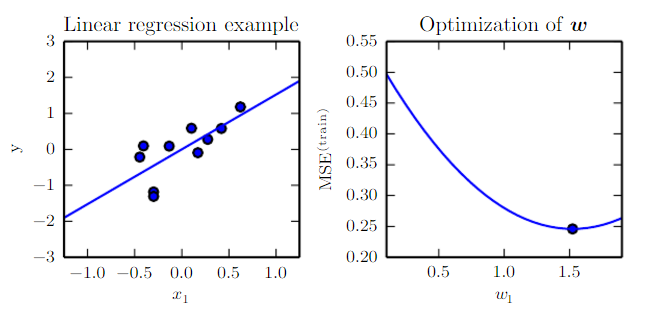
\includegraphics[width=6in]{fig/chap5/5_1.PNG} 
   \caption{图中展示了一个线性回归问题,该问题的训练集中有10个数据点,每个数据点只有一个特征。所以权重向量$w$只有一个需要学习的参数$w_1$ 。(左边)我们设置$w_1$的值使得线$y=w_1x$尽量穿过了所有的数据点。(右边)蓝色的点表示通过标准等式求出来的结果,我们可以看出这个点所代表的权重最小化了训练集中的均方误差。}
   \label{fig:5_1}
\end{figure}

我们需要注意,常用的线性回归的式子比我们刚刚介绍的要复杂一点,模型会加一个新的参数$b$,这是模型就可以这样表示成:
\begin{equation}
  \hat{y}=w^{T}x+b
\end{equation}

这个时候从参数映射到预测值仍然是一个线性过程,但是从特征映射到预测值则是一个仿射变换。增加了这个项之后,我们画出来的图片依然是一条线,但这条线不会经过原点。当然,如果我们不想增加这个偏置项$b$,还是想像之前的模型一样只用一个权重向量,这个时候我们只需要把特征向量$x$增加一维,增加那个维度的值永远设置为$1$。多出的这个新的“特征”所对应的权重取得的效果就和我们刚刚增加的那个偏置项一样。在这本书中我们依然会用“线性(linear)”来表示这类仿射函数。

我们新引入的项$b$通常也叫做仿射变换中的偏置(bias)参数。我们之所以使用这个术语,是因为,当我们啥都不输入或者输入都为$0$的时候,这个仿射变换的输出为$b$,或者说输出偏了$b$。这个偏置和统计学里面的偏差不一样,两者的英语都是bias,统计学中偏差的概念是:统计估计算法对某个值进行估计,但是这个估计的平均值不等于我们所要估计的真实值。

当然,线性回归是一个非常简单而且功能很有限的机器学习算法,但是它向我们展示了机器学习算法是如何运作的。在随后的章节我们会描述设计机器学习算法所需要遵循的一些基本准则,然后会介绍如何利用这些准则来构建更复杂的机器学习算法。

